\documentclass{beamer}

\author[D. Abercrombie]{
  Daniel Abercrombie \\
  Guillelmo Gomez-Ceballos \\
  Benedikt Maier
}

\title{\bf \sffamily Rough Regression}
\date{\today}

\usecolortheme{dove}

\usepackage[absolute,overlay]{textpos}
\usefonttheme{serif}
\usepackage{appendixnumberbeamer}
\usepackage{isotope}
\usepackage{hyperref}
\usepackage[english]{babel}
\usepackage{amsmath}
\setbeamerfont{frametitle}{size=\Large,series=\bf\sffamily}
\setbeamertemplate{frametitle}[default][center]
\usepackage{siunitx}
\usepackage{tabularx}
\usepackage{makecell}
\usepackage{comment}

\setbeamertemplate{navigation symbols}{}
\usepackage{graphicx}
\usepackage{color}
\setbeamertemplate{footline}[text line]{\parbox{1.083\linewidth}{\footnotesize \hfill \insertshortauthor \hfill \insertpagenumber /\inserttotalframenumber}}
\setbeamertemplate{headline}[text line]{\parbox{1.083\linewidth}{\footnotesize \hspace{-0.083\linewidth} \textcolor{blue}{\sffamily \insertsection \hfill \insertsubsection}}}

\IfFileExists{/Users/dabercro/GradSchool/Presentations/MIT-logo.pdf}
             {\logo{\includegraphics[height=0.5cm]{/Users/dabercro/GradSchool/Presentations/MIT-logo.pdf}}}
             {\logo{\includegraphics[height=0.5cm]{/home/dabercro/MIT-logo.pdf}}}

\usepackage{changepage}

\newcommand{\beginbackup}{
  \newcounter{framenumbervorappendix}
  \setcounter{framenumbervorappendix}{\value{framenumber}}
}
\newcommand{\backupend}{
  \addtocounter{framenumbervorappendix}{-\value{framenumber}}
  \addtocounter{framenumber}{\value{framenumbervorappendix}}
}

\graphicspath{{figs/}}

\newcommand{\link}[2]{\href{#2}{\textcolor{blue}{\underline{#1}}}}
\newcommand{\clink}[2]{\link{#1}{http://t3serv001.mit.edu/~dabercro/redir/?k=#2}}}

\newcommand{\twofigs}[4]{
  \begin{columns}
    \begin{column}{0.5\linewidth}
      \centering
      \textcolor{blue}{#1} \\
      \includegraphics[width=\linewidth]{#2}
    \end{column}
    \begin{column}{0.5\linewidth}
      \centering
      \textcolor{blue}{#3} \\
      \includegraphics[width=\linewidth]{#4}
    \end{column}
  \end{columns}
}

\newcommand{\fourfigs}[8]{
  \begin{columns}
    \begin{column}{0.3\linewidth}
      \centering
      \textcolor{blue}{#1} \\
      \includegraphics[width=\linewidth]{#2} \\
      \textcolor{blue}{#3} \\
      \includegraphics[width=\linewidth]{#4}
    \end{column}
    \begin{column}{0.3\linewidth}
      \centering
      \textcolor{blue}{#5} \\
      \includegraphics[width=\linewidth]{#6} \\
      \textcolor{blue}{#7} \\
      \includegraphics[width=\linewidth]{#8}
    \end{column}
  \end{columns}
}

\newcommand{\ttbar}{\ensuremath{t\bar{t}}}
\newcommand{\bbbar}{\ensuremath{b\bar{b}}}

\begin{document}

\begin{frame}
  \titlepage
\end{frame}

\begin{frame}
  \frametitle{Introduction}

  \begin{itemize}
  \item Trained on di-lepton $tt$, but single lepton samples ready
  \item Training using kinematics of
    \begin{itemize}
    \item Jet
    \item Leptons
    \item EM, Charged, Neutral contributions
    \item $\Delta R$ rings
    \item PUPPI components (charged, neutral)
    \end{itemize}
  \item Deep CSV and QGL
  \item Also including event info such as pileup and number of jets
  \item Still throwing together this morning
  \item Using native TensorFlow APIs to allow future flexibility
  \item Will also use TensorFlow for classification
  \end{itemize}

\end{frame}

\begin{frame}
  \frametitle{Model -- Combined}
  \centering
  \includegraphics[width=0.9\linewidth]{full.png}
\end{frame}

\begin{frame}
  \frametitle{Model -- DNN}
  \centering
  \includegraphics[width=0.5\linewidth]{dnn.png}
\end{frame}

\begin{frame}
  \frametitle{Model -- Linear}
  \centering
  \includegraphics[width=0.5\linewidth]{linear.png}
\end{frame}

\begin{frame}
  \frametitle{Loss Function}
  \centering
  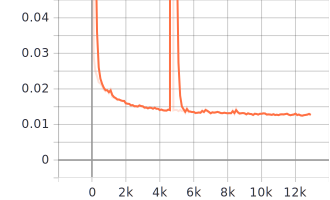
\includegraphics[width=0.7\linewidth]{loss.png}

  Huber loss function \textcolor{red}{$\delta = 1.0$}, will be fixed

\end{frame}

\begin{frame}
  \frametitle{Fraction of Zeros}
  \centering
  \includegraphics[width=0.7\linewidth]{frac.png}
\end{frame}

\begin{frame}
  \frametitle{Regression Results}
  \centering
  \includegraphics[width=0.7\linewidth]{190417_breg_new/hbb_m_tf_v10__hbb_m_tf_v9__hbb_m_tf_v2__hbb_m.pdf}

  DNN, \textcolor{red}{linear}, \textcolor{green}{combined}, \textcolor{blue}{untrained}

\end{frame}

\begin{frame}
  \frametitle{Regression Results -- with $\Delta \eta, \Delta \phi$}
  \centering
  \includegraphics[width=0.7\linewidth]{190417_breg_old/hbb_m_tf_v10__hbb_m_tf_v9__hbb_m_tf_v2__hbb_m.pdf}

  DNN, \textcolor{red}{linear}, \textcolor{green}{combined}, \textcolor{blue}{untrained}

\end{frame}

\begin{comment}
\beginbackup

\begin{frame}
  \frametitle{Backup Slides}
\end{frame}

\begin{frame}
   \frametitle{\small 190813\_testreg\_013/Jet\_puppi\_charged\_ptfrac}
   \centering
   \includegraphics[width=0.6\linewidth]{190813_testreg_013/Jet_puppi_charged_ptfrac.pdf}
\end{frame}

\begin{frame}
   \frametitle{\small 190813\_testreg\_013/Jet\_puppi\_neutral\_ptfrac}
   \centering
   \includegraphics[width=0.6\linewidth]{190813_testreg_013/Jet_puppi_neutral_ptfrac.pdf}
\end{frame}

\begin{frame}
   \frametitle{\small 190813\_testreg\_013/Jet\_puppi\_charged\_pu\_ptfrac}
   \centering
   \includegraphics[width=0.6\linewidth]{190813_testreg_013/Jet_puppi_charged_pu_ptfrac.pdf}
\end{frame}

\begin{frame}
   \frametitle{\small 190813\_testreg\_013/Jet\_puppi\_neutral\_pu\_ptfrac}
   \centering
   \includegraphics[width=0.6\linewidth]{190813_testreg_013/Jet_puppi_neutral_pu_ptfrac.pdf}
\end{frame}

\begin{frame}
   \frametitle{\small 190813\_bukin/signal\_hbb\_m\_190725\_lstm\_pf}
   \centering
   \includegraphics[width=0.6\linewidth]{190813_bukin/signal_hbb_m_190725_lstm_pf.pdf}
\end{frame}

\begin{frame}
   \frametitle{\small 190813\_bukin/signal\_hbb\_m}
   \centering
   \includegraphics[width=0.6\linewidth]{190813_bukin/signal_hbb_m.pdf}
\end{frame}

\begin{frame}
   \frametitle{\small 190813\_bukin/signal\_hbb\_m\_190723\_origin}
   \centering
   \includegraphics[width=0.6\linewidth]{190813_bukin/signal_hbb_m_190723_origin.pdf}
\end{frame}

\begin{frame}
   \frametitle{\small 190813\_bukin/signal\_hbb\_m\_190724\_puppi\_direction}
   \centering
   \includegraphics[width=0.6\linewidth]{190813_bukin/signal_hbb_m_190724_puppi_direction.pdf}
\end{frame}

\begin{frame}
   \frametitle{\small 190813\_ratio/signal\_hbb\_m\_190724\_puppi\_direction}
   \centering
   \includegraphics[width=0.6\linewidth]{190813_ratio/signal_hbb_m_190724_puppi_direction.pdf}
\end{frame}

\begin{frame}
   \frametitle{\small 190813\_bukin/signal\_hbb\_m\_190724\_origin\_direction}
   \centering
   \includegraphics[width=0.6\linewidth]{190813_bukin/signal_hbb_m_190724_origin_direction.pdf}
\end{frame}

\begin{frame}
   \frametitle{\small 190813\_ratio/signal\_hbb\_m\_190724\_origin\_direction}
   \centering
   \includegraphics[width=0.6\linewidth]{190813_ratio/signal_hbb_m_190724_origin_direction.pdf}
\end{frame}

\begin{frame}
   \frametitle{\small 190813\_testreg\_013/Jet\_pf\_0\_transformed\_px}
   \centering
   \includegraphics[width=0.6\linewidth]{190813_testreg_013/Jet_pf_0_transformed_px.pdf}
\end{frame}

\begin{frame}
   \frametitle{\small 190813\_testreg\_013/Jet\_pf\_1\_transformed\_px}
   \centering
   \includegraphics[width=0.6\linewidth]{190813_testreg_013/Jet_pf_1_transformed_px.pdf}
\end{frame}

\begin{frame}
   \frametitle{\small 190813\_testreg\_013/Jet\_pf\_2\_transformed\_px}
   \centering
   \includegraphics[width=0.6\linewidth]{190813_testreg_013/Jet_pf_2_transformed_px.pdf}
\end{frame}

\begin{frame}
   \frametitle{\small 190813\_testreg\_013/Jet\_pf\_3\_transformed\_px}
   \centering
   \includegraphics[width=0.6\linewidth]{190813_testreg_013/Jet_pf_3_transformed_px.pdf}
\end{frame}

\begin{frame}
   \frametitle{\small 190813\_testreg\_013/Jet\_pf\_0\_transformed\_py}
   \centering
   \includegraphics[width=0.6\linewidth]{190813_testreg_013/Jet_pf_0_transformed_py.pdf}
\end{frame}

\begin{frame}
   \frametitle{\small 190813\_testreg\_013/Jet\_pf\_1\_transformed\_py}
   \centering
   \includegraphics[width=0.6\linewidth]{190813_testreg_013/Jet_pf_1_transformed_py.pdf}
\end{frame}

\begin{frame}
   \frametitle{\small 190813\_testreg\_013/Jet\_pf\_2\_transformed\_py}
   \centering
   \includegraphics[width=0.6\linewidth]{190813_testreg_013/Jet_pf_2_transformed_py.pdf}
\end{frame}

\begin{frame}
   \frametitle{\small 190813\_testreg\_013/Jet\_pf\_3\_transformed\_py}
   \centering
   \includegraphics[width=0.6\linewidth]{190813_testreg_013/Jet_pf_3_transformed_py.pdf}
\end{frame}

\begin{frame}
   \frametitle{\small 190813\_testreg\_013/Jet\_pf\_0\_transformed\_pz}
   \centering
   \includegraphics[width=0.6\linewidth]{190813_testreg_013/Jet_pf_0_transformed_pz.pdf}
\end{frame}

\begin{frame}
   \frametitle{\small 190813\_testreg\_013/Jet\_pf\_1\_transformed\_pz}
   \centering
   \includegraphics[width=0.6\linewidth]{190813_testreg_013/Jet_pf_1_transformed_pz.pdf}
\end{frame}

\begin{frame}
   \frametitle{\small 190813\_testreg\_013/Jet\_pf\_2\_transformed\_pz}
   \centering
   \includegraphics[width=0.6\linewidth]{190813_testreg_013/Jet_pf_2_transformed_pz.pdf}
\end{frame}

\begin{frame}
   \frametitle{\small 190813\_testreg\_013/Jet\_pf\_3\_transformed\_pz}
   \centering
   \includegraphics[width=0.6\linewidth]{190813_testreg_013/Jet_pf_3_transformed_pz.pdf}
\end{frame}



\backupend
\end{comment}

\end{document}
